\begin{frame}
\frametitle{Corps humain / Description}
\begin{columns}
\column{0.55\textwidth}
\scalebox{0.8}{\begin{minipage}{1.25\textwidth}
\begin{itemize}
\item 12 organes dont le squelette ;
\item $5\,840\,122$ tétraèdres découpés ;
\item Permittivités relatives : Gabriel, 1996 ;
\item Condition limite absorbante (PML de Bérenger) ;
\item Antenne Bluetooth rayonnant à 2.45 GHz ;
\item Facteur d'échelle d'ordre 1300 ;
\item Forme d'onde (6 ns) : Gaussienne modulée.
\end{itemize}
\end{minipage}}
\vskip-1em
\begin{columns}
\column{0.5\textwidth}
\scalebox{0.7}{\begin{minipage}{1.42\textwidth}
\begin{figure}
	\centering
		\begin{tabular}{|c|c|c|c|c|}
			\hline
			Matériau & $\EPrm_r$\\ \hline\hline
			cerveau & $48.34$ \\	\hline
			cœur & $58.67$ \\	\hline
			poumon & $22$ \\	\hline
			foie & $41.82$ \\	\hline
			bile & $60$ \\	\hline
			rate & $56.75$ \\	\hline
			pancréas & $56.75$ \\	\hline
			rein & $56.83$ \\	\hline
			colon & $48.5$ \\	\hline
			vessie & $20$ \\	\hline
			muscle & $50$ \\	\hline
			os & $11.41$ \\	\hline
			cartilage & $36$ \\	\hline
			vide & $1$ \\	\hline
		\end{tabular}
\end{figure}
\end{minipage}}
\column{0.5\textwidth}
\begin{figure}
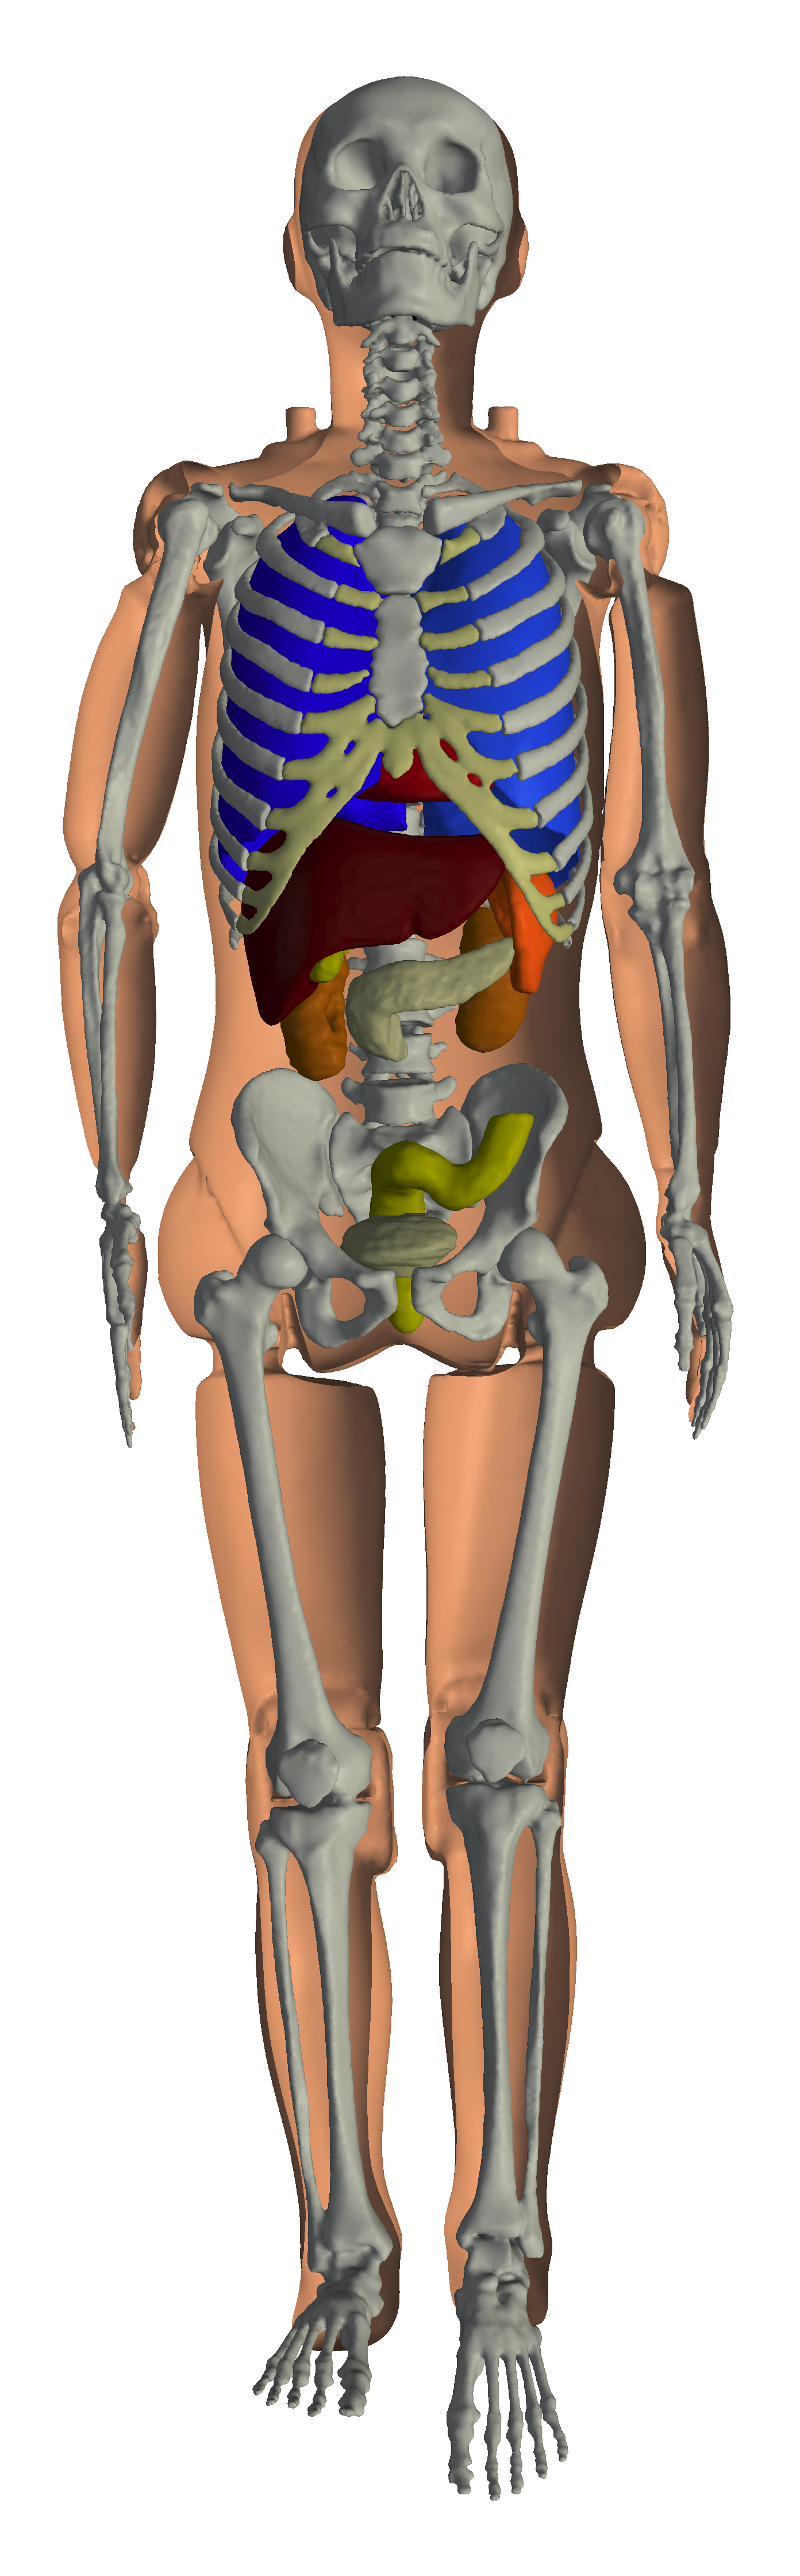
\includegraphics[width=0.5\textwidth]{../img/kyoto}
\end{figure}
\end{columns}
\column{0.45\textwidth}
\vskip-1em
\begin{figure}
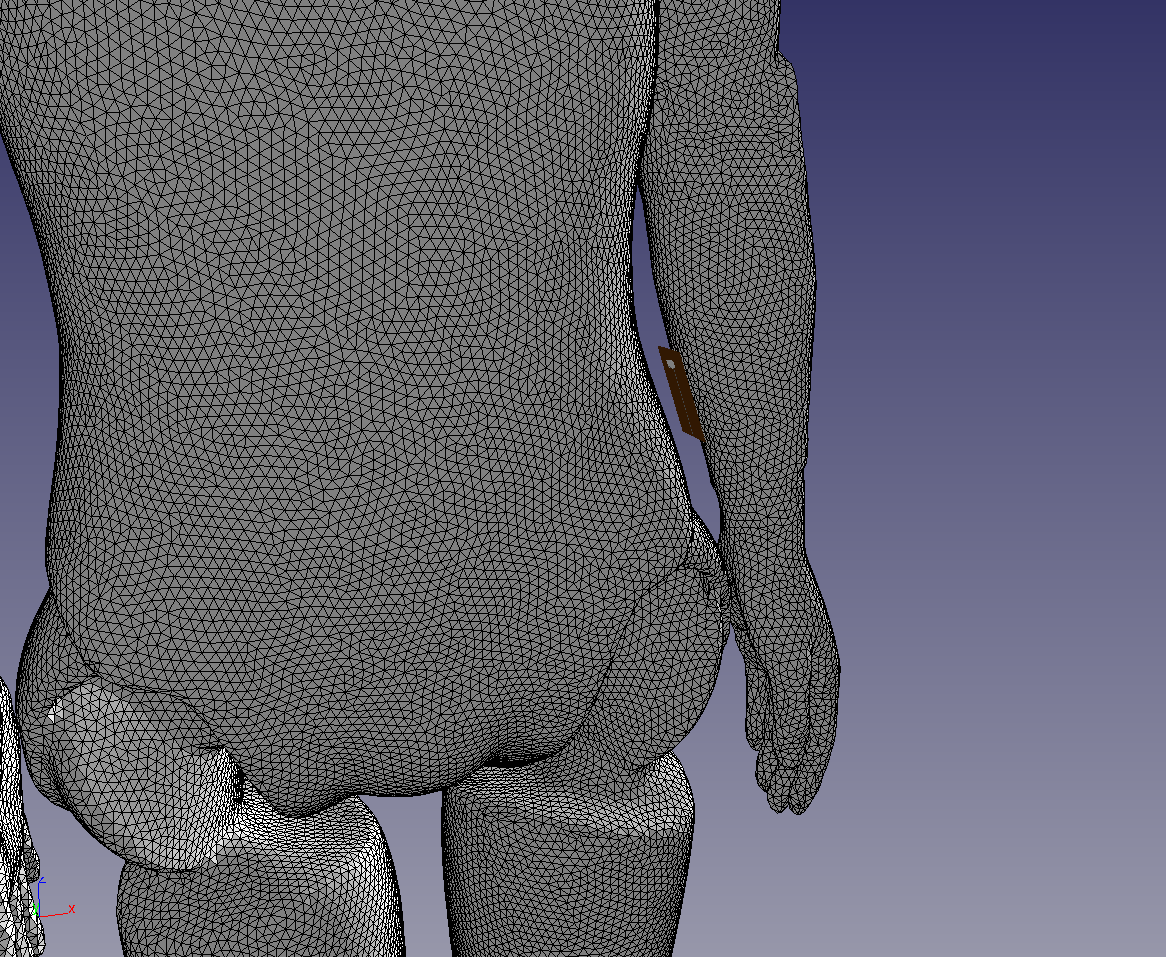
\includegraphics[width=0.8\textwidth]{../img/wide_ltcc}
\end{figure}
\vskip-1em
\begin{figure}
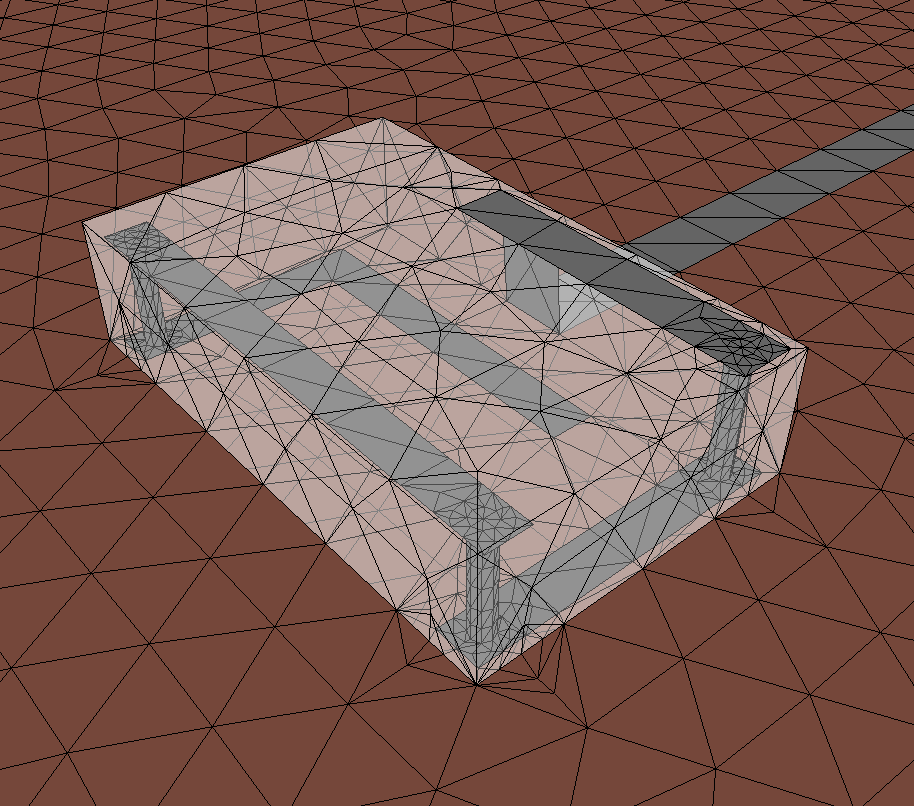
\includegraphics[width=0.8\textwidth,
%trim={0 200 0 200},clip
]{../img/ltcc}
\end{figure}
\end{columns}
\vfill
\end{frame}

